\documentclass[tikz]{standalone}

\usetikzlibrary{shapes}
\usetikzlibrary{angles}
\usetikzlibrary{calc} 

\usetikzlibrary{decorations.pathreplacing}
\usetikzlibrary{decorations.markings}
\usetikzlibrary{decorations.text}

\usetikzlibrary{shapes.geometric}


% This bascially automates a \newcommand{<name>}{} to ensure
% that a command with the given <name> does not already exist
\providecommand*{\pgfmathsetnewmacro}[2]{%
    \newcommand*{#1}{}% Error if already defined
    \pgfmathsetmacro{#1}{#2}%
}%


\begin{document}
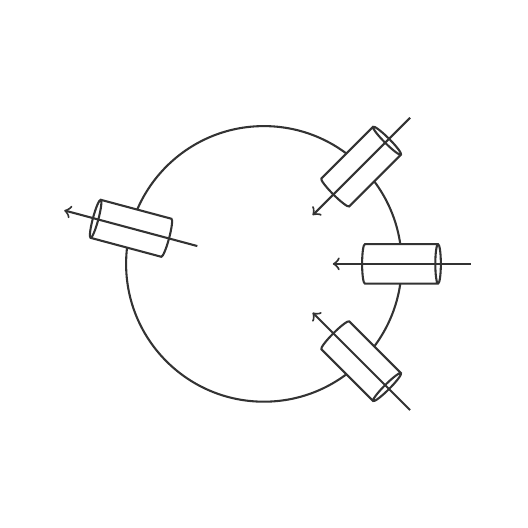
\begin{tikzpicture}[black!80, line width = 0.75pt]

\pgfmathsetnewmacro{\bb}{3}
\useasboundingbox[clip] (-\bb,-\bb) rectangle (\bb,\bb);


\pgfmathsetnewmacro{\radius}{1.75}
\pgfmathsetnewmacro{\length}{0.5}



\coordinate (O) at (0,0);

\draw (O) circle (\radius);


%\providecommand\drawChannel#1#2#3




\foreach \ANGEL/\LABEL/\DIRECTION in {
                        000/ a /{<-},
                        045/ b /{<-},
                        315/ d /{<-},
                        165/ c /{->}}{
    \path (O) -- ($(O)!0.99!(\ANGEL:\radius)$) 
        node [pos = 0.99, 
              sloped, 
              cylinder, 
              draw = black!80, fill = white, 
              minimum height=2cm,
              minimum width=1cm,
              aspect = .60,
              transform shape,
              allow upside down= true,
              scale = \length] {};
    \draw[\DIRECTION] ($(O)!0.50!(\ANGEL:\radius)$) -- ($(O)!1.50!(\ANGEL:\radius)$); 
    };
    
\end{tikzpicture}
\end{document}